%!TEX root = ../lectures_olympics.tex

\chapter{波动光学}

历史上们始终就光的本性有着长期的争论,{\heiti 牛顿}({\it I. Newton})在万有引力理论的基础上提光的{\heiti 微粒学说}(particle theory),认为光是由不同颜色的微小颗粒构成;与之相对的以{\heiti 惠更斯}({\it C. Huygens})为代表的{\heiti 波动学说}(wave theory)是其有力的竞争者。
起初颗粒学说占据上风,但随着光的干涉、衍射现象的发现对颗粒说造成了冲击,我们慢慢知道,光其实就是电磁波,在电磁学的基础上证实了光的波动性。
因为光的波动本性,自然会有大量的与其波动性相关实验现象和理论,并有着广泛的应用,它们是本章将要学习的主要内容,他们都基于光的{\heiti 电磁学说}(electromagnetic theory)。
事实上光的电磁学说建立不久,新的实验现象就对其提出了挑战,这些现象将在后面给出。它使人们开始意识到光的{\heiti 波粒二象性}(wave-particle duality)。从而发展出光的{\heiti 量子学说}(quantum theory)。


\section{干涉}
根据光的电磁学说,沿直线传播的光可以看成是一列平面电磁波,它的性质可由电磁波的振幅、振动方向\footnote{因为电磁波是横波,所以平面电磁波有两个独立的振动方向}、频率和相位共同决定,并且在传播过程中满足电磁场的一般规律。
这其中最重要的规律之一就是叠加原理,它指出不同源产生的电磁场对空间中同一点的贡献等于两个源产生电场和磁场的矢量和,也就是说当两束光相遇时空间中真实的电磁场是两束光对应的电、磁场的叠加。
此外对于可见光来说,它们对应电磁波的频率极其之高,远超出肉眼甚至仪器的灵敏度,所以对光的观测实际上并不能够测量空间中任何一点电磁场的瞬时值,而是场的某种平均值。
和通常的机械波类似最容易测量的是波的能量,或更准确地说是波的能量密度,对于电磁波来说它在空间中一点的能量密度的瞬时值正比于电磁波振幅的平方,而能量密度的平均值则是振幅平方的时间平均值,如果电磁波是可见光范围,其能量密度的时间平均值对应于人眼或光学仪器记录到的光的明暗。

根据以上两点可以立刻做出推论:当两束具有相同频率、相同振动方向和固定相位差的光在空间中相遇时,其交叠区域会产生交替出现的明、暗条纹,在有的地方光亮度增强,而在有的地方亮度减弱。
其实这种现象早在1807年就由英国物理学家托马斯$\cdot$杨({\it T. Young})通过称之为光的{\heiti 双缝干涉实验}(double-slit interference experiment)所发现。
其实验原理如图\ref{fig:wave-optics-2}(a)所示,一束光通过狭缝$S_1$以后再分别通过狭缝$S_2$和$S_3$以后在光屏$F$上相遇,观测结果表明在光屏$F$上形成如侧所示的明暗相间的条纹。

\begin{figure}
\centering
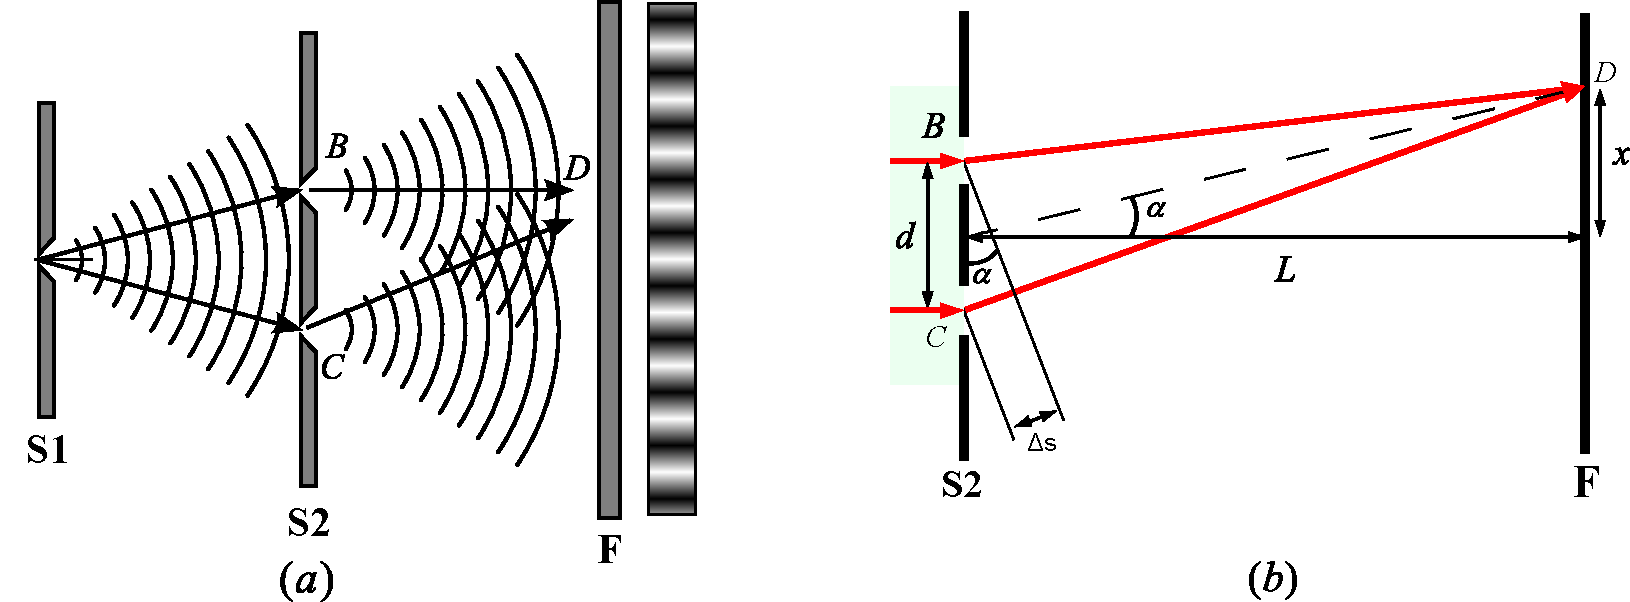
\includegraphics[width=0.7\linewidth]{images/wave-optics-2}
\caption{(a)双缝干涉实验示意图(b)各个几何量的定义}
\label{fig:wave-optics-2}
\end{figure}

假设实验光束可以看做波长为$\lambda$的单色光,狭缝B、C之间的距离为$d$,双缝至光屏F的距离为$L$,我们看距离光屏中线$x$距离处D点的光强,如图\ref{fig:wave-optics-2}(2)所示。
因为B、C两点与A距离相同,可以认为两点上发出的光具有相同的振幅和相位。
当$x\neq 0$时,D点与其到B、C两点的距离不同,从两狭缝发出的光在D点相遇时会有一定的相位差。
假设双缝间距$d$和$x$与$L$相比很小,则根据几何关系可知
\begin{eqnarray*}
\overline{\rm BD}& =& \sqrt{L^2+\left(x-\frac{d}{2}\right)^2}\simeq L + \frac{(x-d/2)^2}{2L}\\
\overline{\rm CD}& =& \sqrt{L^2+\left(x+\frac{d}{2}\right)^2}\simeq L + \frac{(x+d/2)^2}{2L}
\end{eqnarray*}
由此得出两束光线距离的差
\[
\Delta S = \overline{\rm CD}-\overline{\rm BD} = \frac{d}{L}x = d\sin\alpha,
\]
其中$\alpha$角的定义由图\ref{fig:wave-optics-2}(b)中给出。
因为两束光线行进的距离不同,在D点相遇时有相位差
\[\Delta\varphi = \frac{\Delta S}{2\pi\lambda} = \frac{xd}{ L\lambda}2\pi,\]
假设光的振幅为$A$,那么在D点场强随时间的变化关系可以示意性地由
\[
A+A\cos\Delta\varphi = 2A\cos^2\frac{\Delta \varphi}{2} = 2A^2\cos^2\frac{xd}{\lambda L}\pi,
\]
根据三角函数的性质可知当
\[ \frac{xd}{\lambda L}\pi = n\pi,\qquad x = n\frac{L}{d}\lambda,\qquad n = 0,\pm 1,\pm 2\cdots \]
时振幅有极大值,此时对应于亮条纹,对应的整数$n$称为{\heiti 干涉级数}(interference order),尤其是对应于$n=0$的亮条纹,它位于双缝正中,实验上它也最亮。
反之当
\[ \frac{xd}{\lambda L}\pi = (n+\frac{1}{2})\pi,\qquad x =(n+\frac{1}{2})\frac{L}{d}\lambda,\qquad n = 0,\pm 1,\pm 2\cdots \]
时振幅为零,对应于暗条纹。
根据条纹的分布和各个几何量以及光波长的关系可以得到以下结论:
\begin{itemize}
\item 理想情况下对于波长为$\lambda$的单色光源,双缝干涉条纹等间距分布,与干涉级数无关,相邻两条明、暗条纹之间的距离
\begin{equation}
\Delta x = \frac{L}{d}\lambda,
\end{equation}
可见双缝离屏越远、双缝间距越小,所用光源波长越长则条纹间距越大,反之条纹间距越小。
\item
上式可以用来测量光的波长,只需通过实验装置的摆放确定$L$和$d$,再通过测量得到条纹的间距$\Delta x$,这样可得实验光源的波长
\begin{equation}
\lambda = \frac{d}{L}\Delta x.
\end{equation}
\item 
如果光源是白光,因为它是由多种颜色的光混合而成,所以除了中央亮条纹以外其余各级条纹会出现彩色。
\end{itemize}

在应用以上结论讨论实际问题时,还应当注意以下几件事情。
双缝实验中缝的宽度越小,则干涉条纹就越清晰、越明亮,反之缝越宽则干涉条纹则越模糊,这时因对如果缝过宽,通过它的不同部位到达光屏上给定点的光的光程有一定的弥散,缝越宽则弥散越大,影响了条纹的清晰度。
另外,并不是对于任意大的$n$都能够看到其干涉条纹,这与光源所发光的性质有关,对于普通的光源的双缝实验只能够看到最低的几级干涉条纹,而如果将光源换成激光则有机会看高更高级的条纹。
当相干光束的亮度判别过大时虽然理论计算可知亮度有周期性的变化,但实际亮度的变化比起光本身的强度的区别度过小,也无法观察干涉效应。作为高频电磁波的光的干涉条件较机械波干涉更为衍射,它要求一个更严格的{\heiti 相干性}(quality of coherence)。













%%%%%%%%%%%%%%%%%
\begin{example}

在双缝干涉装置中,双缝间距为$0.2\unit{mm}$,单缝位于双缝的中垂线上,屏与双缝的距离为$1.0\unit{m}$。
如果用某单色光源照射,从光屏上测得第4级明条纹到中央明条纹的距离为$1\unit{cm}$。
求该单色光的波长。

如果把其中的一条缝用厚度为$4.5\unit{\mu m}$的透明板挡住,结果发现第4级条纹移到中央明条纹的位置,则该透明板的折射率为多少?
\tagged{student}{\vspace*{4cm}}
\begin{taggedblock}{teacher}

解析:单色光的波长根据前面的公式直接得出
\[
\lambda = \frac{d}{L}\Delta x = 5\pow{-7}\unit{m},
\]
设透明板的折射率为$n$,厚度为$t$,那么通过它光程将增加$\Delta s = (n-1)t$,它导致的相位差为$4.5\cdot 2\pi$,这样
\[
n=1+\frac{4.5\lambda}{t}  = 1.5
\]
\end{taggedblock}
\end{example}
%%%%%%%%%%%%%%%%%%%%%%






%%%%%%%%%%%%%%%%%
\begin{example}
	用单色光作如图所示的双缝干涉实验时,位置的调节很难作得完全精确。
	
	1. 如果光源前狭缝$S$(看做线光源)的位置向中线$OO'$的一侧偏离了一个小距离,则与调节精确时相比,观察屏$E$上的条纹间距\kong\kong(变大,变小或不变)。
	
	2. 如果观察屏$E$(垂直于图面)与它的正确位置成一个小角度,则与调节精确时相比,屏上的条纹间距\kong\kong(变大,变小或不变)。
	\begin{flushright}
		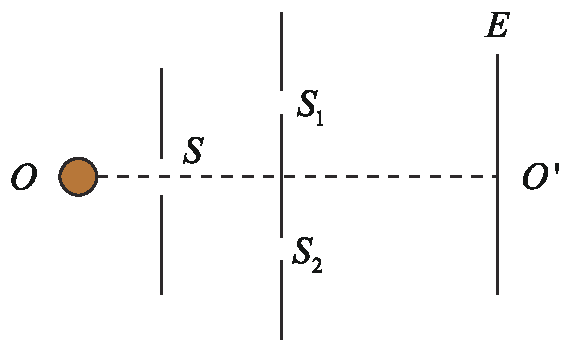
\includegraphics[width = 0.4\textwidth]{images/wave-optics-5.pdf} 
	\end{flushright}
	\tagged{student}{\vspace*{0cm}}
	\begin{taggedblock}{teacher}
		
		解析:不变,变大。利用干涉条纹出现的条件以及空间分布即可判断。
	\end{taggedblock}
\end{example}
%%%%%%%%%%%%%%%%%%%%%%

%%%%%%%%%%%%%%%%%
\begin{example}
传统的雷达天线依靠转动天线来搜索空中各个方向的目标,这严重影响了搜索的速度。
现代的“雷达”是“相位控制阵列雷达”,它是由数以万计的只有几厘米或更小的小天线按一定的顺序排列成的天线阵,小天线发出相干的电磁波,其初相位可通过电子计算机调节,从而可改变空间干涉极强的方位,这就起了快速扫描搜索空中各个方向目标的作用。
对下面的简单模型的研究,有助于了解改变相干波的初相位差对空间干涉极强方位的影响。
图中$a、b$为相邻两个小天线,间距为$d$,发出波长为$\lambda$的相干电磁波。$Ox$轴通过$a$、$b$的中点且垂直于$a$、$b$的连线。
若已知当$a$、$b$发出的电磁波在$a$、$b$处的初相位相同即相位差为O时,将在与$x$轴成$\theta$角($\theta$很小)方向的远处形成干涉极强,现设法改变$a$、$b$发出的电磁波的初相位,使$b$的初相位比$a$的落后一个小量$\varphi$,结果,原来相干极强的方向将从$\theta$变为$\theta'$,则$\theta-\theta' = \underline{\qquad \qquad }$。
\begin{flushright}
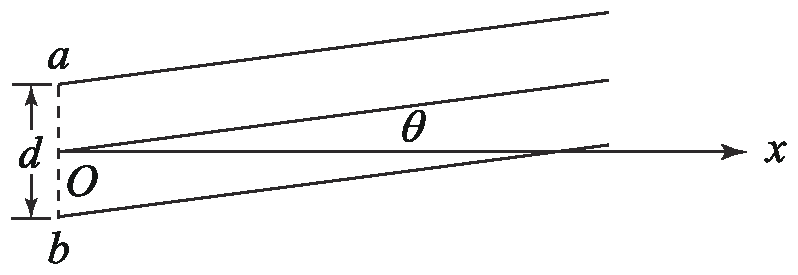
\includegraphics[width = 0.6\textwidth]{images/wave-optics-1.pdf} 
\end{flushright}


\tagged{student}{\vspace*{2cm}}
\begin{taggedblock}{teacher}

解析:角度改变意味着光程的变化,从已知量可以光程的变化量$d(\theta-\theta')$,而这个变化可由两束光相位的变化抵消,当相位差为$\varphi$时我们有
\[
d(\theta-\theta')=\frac{\varphi}{2\pi}\lambda,\qquad \theta-\theta' = \frac{\varphi \lambda}{2\pi d}.
\]
\end{taggedblock}
\end{example}
%%%%%%%%%%%%%%%%%%%%%%

%%%%%%%%%%%%%%%
\begin{example}
	如图所示,波长为$\lambda$的平行激光束垂直入射到双棱镜上,双棱镜的顶角为$\alpha\ll 1$,宽度为$D$,折射率为$n$,在双棱镜后方能否看到激光的干涉图样,如果有的话在什么区域内能够观察到它们,条纹间距又是多少?
			\begin{flushright}
				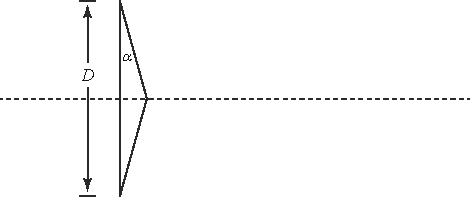
\includegraphics[width = 0.5\textwidth]{images/wave-1.pdf}
			\end{flushright}
	\tagged{student}{\vspace*{4cm}}
	\begin{taggedblock}{teacher}
		
		解析:上下方折射光交叠的区域内可以发生干涉,区域为棱前角度为$2(n-1)\alpha$的角内。条纹间距$\Delta x = \frac{\lambda}{2(n-1)\alpha}$
	\end{taggedblock}
\end{example}%%%
%%%%%%%%%%%%%%$$

%%%%%%%%%%%%%%%
\begin{example}
	将焦距$ f=20\si{cm}$的凸薄透镜从正中切去宽度为$ a $的小部分,见图 (a).再将剩下的两半粘接在一起,构成一个“粘合透镜”,见图 (b).图中$ D=2\si{cm}$,在粘合透镜一侧的中心轴线上距镜$ 20\si{cm}$处,置一波长$\lambda=500\si{nm}$的单色点光源$ S$,另一侧垂直于中心轴线放置屏幕,见图 (c).屏幕上出现干涉条纹,条纹间距$\Delta x = 0.2\si{mm}$,试问:
	
	 1.切去部分的宽度 $a $是多少?
	 
	 2.为获得最多的干涉条纹,屏幕应离透镜多远?
	 		\begin{flushright}
	 			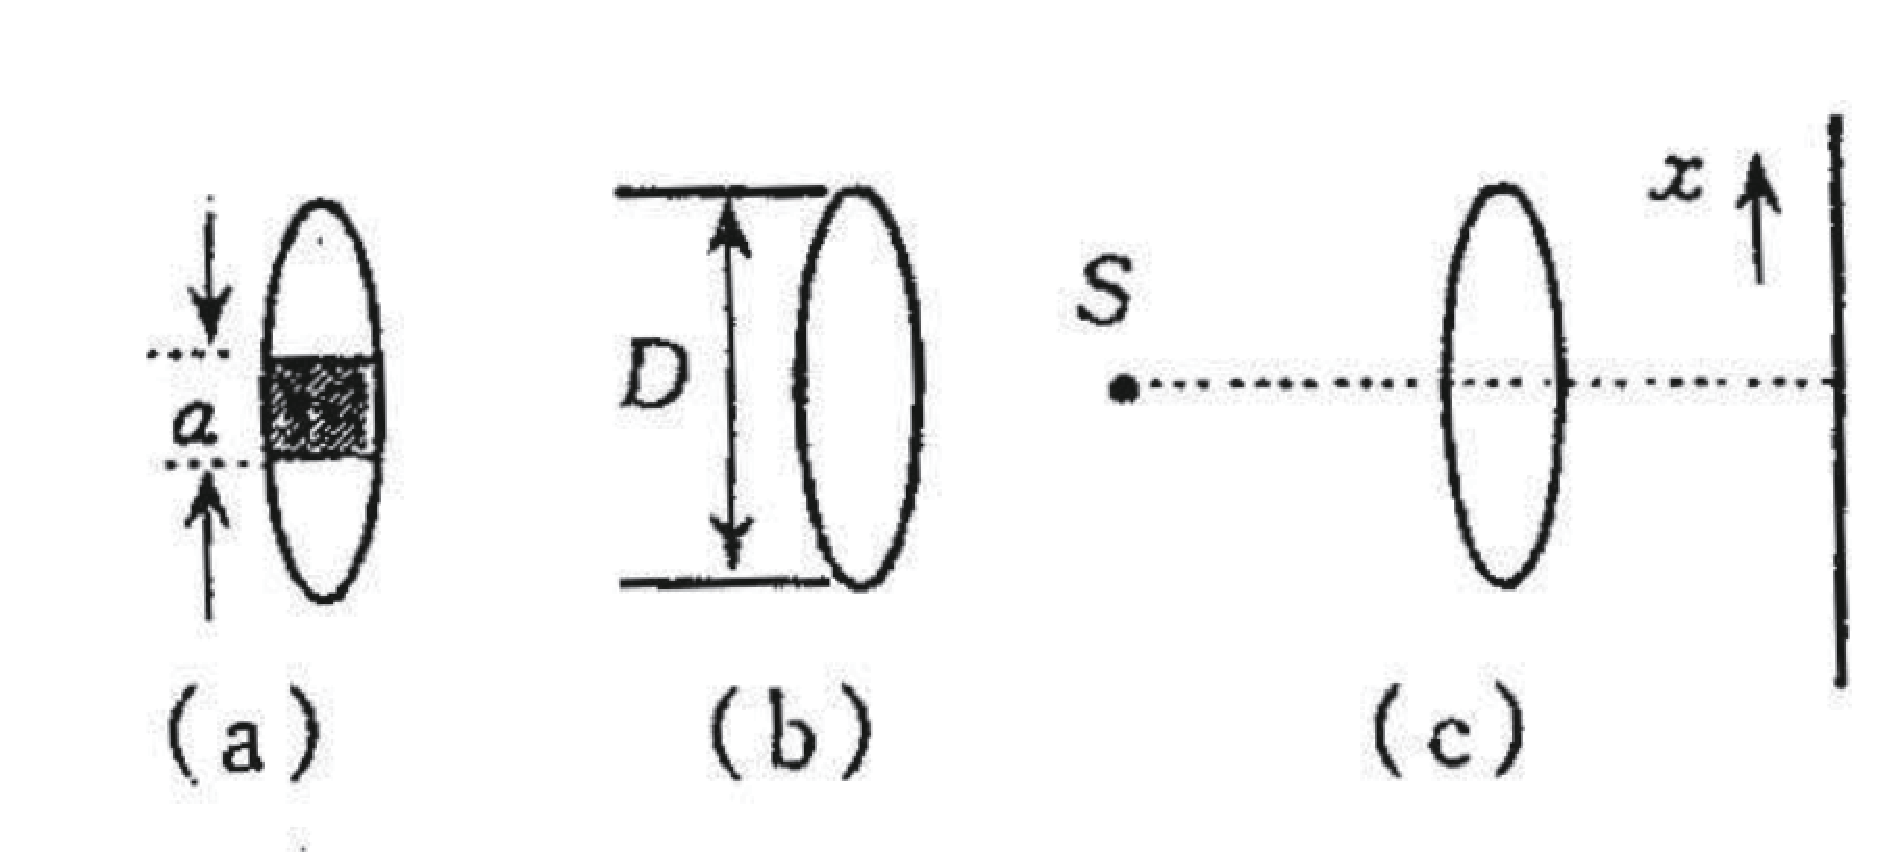
\includegraphics[width = 0.4\textwidth]{images/wave-optics-10.pdf} 
	 		\end{flushright}
	\tagged{student}{\vspace*{4cm}}
	\begin{taggedblock}{teacher}
		
		解析:1. $a=\frac{\lambda f}{\Delta x}=0.5\si{mm}$\\
		2. $L= \frac{Df}{2a} = 4\si{m}$
	\end{taggedblock}
\end{example}%%%
%%%%%%%%%%%%%%$$



%%%%%%%%%%%%%%%
\begin{example}
	如图所示的洛埃镜镜长$ l=7.5\si{cm}$,点光源$ S $到镜面的距离$ d=0.15\si{mm}$,到镜面左端的距离$b=4.5\si{cm}$,光屏$ M $垂直于平面镜且与点光源$ S $相距$ L=1.2\si{m}$。如果光源发出长$\lambda = \num{6e-7}\si{m}$的单色光,求:
	
	(1)在光屏上什么范围内有干涉的条纹? 
	
	(2)相邻的明条纹之间距离多大? 
	
	(3)在该范围内第一条暗条纹位于何处?
			\begin{flushright}
				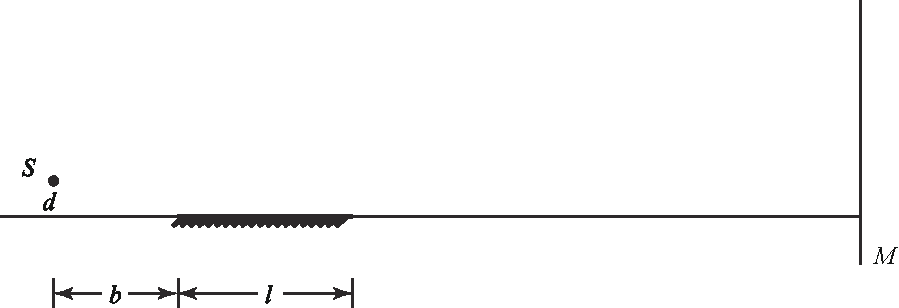
\includegraphics[width = 0.5\textwidth]{images/wave-optics-9.pdf} 
			\end{flushright}
	\tagged{student}{\vspace*{4cm}}
	\begin{taggedblock}{teacher}
		
		解析:(1) $y \sim 1.35\si{mm} -- 3.85\si{mm}$\\
		(2) $2.4mm$\\
		(3) $y=2.4mm$
	\end{taggedblock}
\end{example}%%%
%%%%%%%%%%%%%%$$







%%%%%%%%%%%%%%%%%
\begin{example}
	一斜劈形透明介质劈尖,尖角为$\theta$,高为$h$。
	今以尖角顶点为坐标原点,建立坐标系如左图所示;劈尖斜面实际上是由一系列微小台阶组成的,在左图中看来,每一个小台阶的前侧面与$xz$平面平行,上表面与$yz$平面平行。
	劈尖介质的折射率$n$随$x $而变化,$n(x)=1+bx$,其中常数$b>0$。
	一束波长为$\lambda$的单色平行光沿$x$轴正方向照射劈尖;劈尖后放置一薄凸透镜,在劈尖与薄凸透镜之间放一档板,在档板上刻有一系列与$z$方向平行、沿$y$方向排列的透光狭缝,如右图所示。
	入射光的波面(即与平行入射光线垂直的平面)、劈尖底面、档板平面都与$x$轴垂直,透镜主光轴为$x$轴。
	要求通过各狭缝的透射光彼此在透镜焦点处得到加强而形成亮纹。 已知第一条狭缝位于$y=0$处;物和像之间各光线的光程相等。 
	
	1. 求其余各狭缝的$y$坐标;
	
	2. 试说明各狭缝彼此等距排列能否仍然满足上述要求。
	\begin{flushright}
		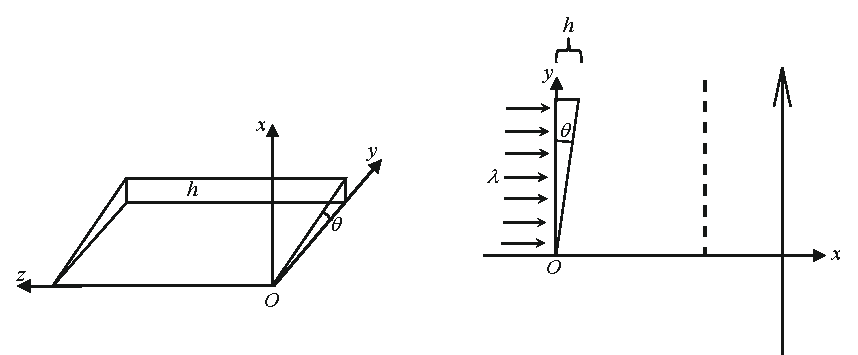
\includegraphics[width = 0.7\textwidth]{images/wave-optics-4.pdf} 
	\end{flushright}
	\tagged{student}{\vspace*{4cm}}
	\begin{taggedblock}{teacher}
		
		解析:题目很长,但仔细分析以后其实并不复杂。
		透镜成像本身就是等光程的,所以实际上只需要计算到达透镜之前的光程并令它们相等即可。
		从$x=0$入射到某一$x$出射,光所经历的光程
		\[
		\int_0^xndx = \int_0^x (1+bx)dx = x + \frac{1}{2}bx^2
		\]
		再加上剩下部分的光程,总的光程为
		\[
		x + \frac{1}{2}bx^2+(L-x) = L+\frac{1}{2}bx^2.
		\]
		根据题意它们需要是$y=0$光线光程相差波长的整数倍:
		\[
		L+\frac{1}{2}bx^2 = L+n\lambda ,\qquad x = \sqrt{\frac{2n\lambda}{b}}.
		\]
		再根据几何关系可知$y = x\cot \theta$,这样缺口的$y$坐标应当满足:
		\[
		y_n = \sqrt{2\lambda/b}\cot\theta\sqrt{n},\qquad n=0,1,2\cdots 
		\]
		从中也可看出,等间距分布时也会达到相同的效果。
	\end{taggedblock}
\end{example}
%%%%%%%%%%%%%%%%%%%%%%


%%%%%%%%%%%%%%%
\begin{example}
	【思考】若在杨氏双缝干涉实验中,直接采用两个狭缝型的独立光源C和D\ref{fig:wave-optics-2}。可否观察到同样的实验现象?
	\tagged{student}{\vspace*{2cm}}
	\begin{taggedblock}{teacher}
		
		解析:除非光源C和D为激光光源,否则由于光源C和D之间的相位差并不能稳定而没有干涉条纹。
	\end{taggedblock}
\end{example}%%%
%%%%%%%%%%%%%%$$



除了双缝干涉以外还有一类典型的干涉现象称为{\heiti 薄膜干涉}(thin-film interference),在地表的油膜或者肥皂泡上很容易看到薄膜干涉现象。
当光射到一透明薄膜上时,薄膜的上、下两个表面都会不同程度地将光反射,当上、下表面的反射光相遇时会互相干涉。
处理薄膜干涉的数学方法和双缝干涉没有本质的不同,但要注意光波在反射过程中一个现象:{\heiti 半波损失}(half-wave loss):当光由折射率较小的介质射向折射率较大的介质,在两介质表面发生反射时其相位会有一个突变,其大小刚好为$\pi$,故称此现象为半波损失,从介质表面反射光的电场强度表达中也可定量地看出这一现象。
如果单色光在空气中波长为$\lambda$,薄膜厚度为$d$时,两束光在上表面的相位差
\[
\Delta \varphi = \pi + \frac{2dn}{\lambda}2\pi
\]
简单的分析可知当
\begin{equation}
d  = \frac{\lambda}{2n}(N+\frac{1}{2}),\qquad N = 0,1,2\cdots
\end{equation}
时会有干涉极强,而当
\begin{equation}
d = \frac{\lambda}{2n}N,\qquad N = 1,2,3\cdots
\end{equation}
时则会出现干涉相消。

%%%%%%%%%%%%%%%%%
\begin{example}
	
	有些相机和测量仪器的镜头看上去是紫红(或蓝紫)色的,这是因为镜头表面镀了一层透明物质的薄膜,它的作用是什么?
	\tagged{student}{\vspace*{2cm}}
	\begin{taggedblock}{teacher}
		
		解析:增透黄绿色光
	\end{taggedblock}
\end{example}
%%%%%%%%%%%%%%%%%%%%%%






%%%%%%%%%%%%%%%
\begin{example}
	一束白光以$30^\circ$角射在肥皂膜上,反射光中波长$\lambda = 500\si{nm}$的绿光显得特别明亮,肥皂膜液体的折射率$ n=1.33$。 
	
	1、试问薄膜最小厚度为多少?
	
	2、从垂直方向观察,薄膜是什么颜色?
	\tagged{student}{\vspace*{4cm}}
	\begin{taggedblock}{teacher}
		
		解析:1、 推导斜角度薄膜干涉的光程差公式
		\[\delta = 2nd \cos \theta\]
		考虑半波损失,得$d_{min}=108nm$\\
		2、 正入射对应的干涉相长波长$\lambda^\prime = 577\si{nm}$。这是黄光。
	\end{taggedblock}
\end{example}%%%
%%%%%%%%%%%%%%$$


%%%%%%%%%%%%%%%%%
\begin{example}
	
	用光的干涉原理可以精确地测量金属丝的直径,装置如图所示,待测金属丝置于两块平晶的一端,金属丝与平晶交界线距离为$L$。
	测量时用波长为$\lambda$的单色光垂直入射,并测得两条亮条纹的间距为$l$,求金属丝的直径$D$。
	\begin{flushright}
		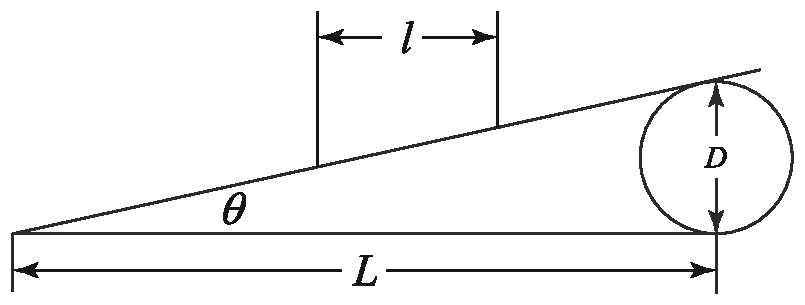
\includegraphics[width = 0.4\textwidth]{images/wave-optics-3.pdf} 
	\end{flushright}
	\tagged{student}{\vspace*{2cm}}
	\begin{taggedblock}{teacher}
		
		解析:一般来说金属丝的直径极其之小,由于它的存在导致图中的$\theta = \frac{D}{L}$,这样相距$l$距离上的高度差$\Delta h = l\theta = l\frac{D}{L}$,这个高度差导致光程相差一个波长:
		\[
		2l\frac{D}{L} = \lambda,\qquad D = \frac{L\lambda}{2l}
		\]
	\end{taggedblock}
\end{example}
%%%%%%%%%%%%%%%%%%%%%%

%%%%%%%%%%%%%%%
\begin{example}
某射电天文台的接收天线位于海平面上方高度为$h = 2\si{m}$处,接收机只记录电场强度的水平分量。
当一颗能发射波长为$\lambda = 21\si{cm}$电磁波的射电星从海平面升起时,接收机将相继地记录下一系列极大值和极小值。

1. 试确定观察到极大值和极小值时电磁波的方向,用与海平面的夹角表示。

2. 当射电星从海平面上方出现时,试问接收到的电磁波强度是增大还是减小?

3. 试求观察到的相继各极大值与极小值的相对强度。
	\tagged{student}{\vspace*{4cm}}
	\begin{taggedblock}{teacher}
		
		解析:极大值产生的条件
		
		\[\sin\theta_{max} = \frac{\lambda}{2h}(k-1/2),\]
		极小值则是
			\[\sin\theta_{min} = \frac{\lambda}{2h}(k),\]
			刚升起时电场强度逐渐增加。
	\end{taggedblock}
\end{example}%%%
%%%%%%%%%%%%%%$$

%%%%%%%%%%%%%%%
\begin{example}
	牛顿曾观察到一束细日常射到有灰尘的反射镜上面会产生干涉条纹。
	为了分析这一现象背后的物理,考虑如图所示的简单实验。
	一平板玻璃的折射率为$n$,厚度为$t$,下表面涂有水银反射层,上表面撒有滑石粉(灰尘粒子)。
	观察者$O$和单色光源$L$(光线的波长为$\lambda$)的连线垂直于镜面(垂足为$N$),$LN=a$,$ON=b$。
	反射镜面上的某灰尘粒子$P$与直线$ON$的距离为$r$($b>a\gg r>t$)。
	观察者可以观察到明暗相间的环形条纹。
	
	(1) 求第$m$个亮环到$N$点的距离;
	
	(2) 若$n=1.63, a=0.0495\si{m},b=0.245\si{m},t = \num{1.1e-5}\si{m},\lambda=680\si{nm}$,求最小亮环$m=1$的半径。
			\begin{flushright}
				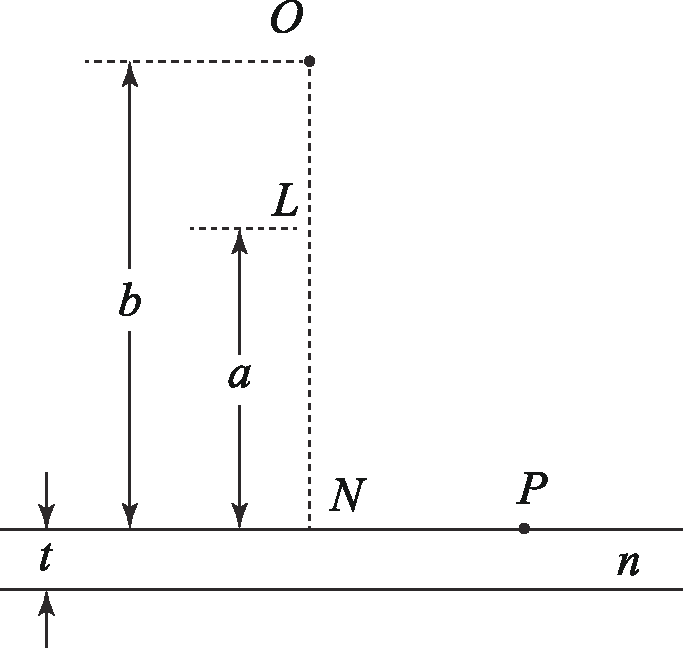
\includegraphics[width = 0.3\textwidth]{images/wave-optics-8.pdf} 
			\end{flushright}
	\tagged{student}{\vspace*{2cm}}
	\begin{taggedblock}{teacher}
		
		解析:2016初赛倒数第二题。
	\end{taggedblock}
\end{example}%%%
%%%%%%%%%%%%%%$$


%%%%%%%%%%%%%%%
\begin{example}
	在一块光平的玻璃片$ B上$,放曲率半径$ R$很大的平凸透镜$ A$,在$ A$、$B$之间形成一劈尖形空气薄层。当平行光束垂直地射向平凸透镜时,可以观察到在透镜表面出现一组干涉条纹,这些干涉条纹是以接触点$ O$为中心的同心圆环,称为牛顿环。
	求各个亮环中心距离中心的半径。
	\tagged{student}{\vspace*{4cm}}
	\begin{taggedblock}{teacher}
		
		解析:\[
		r_k = \sqrt{\frac{2k-1}{2}R\lambda}
		\]
	\end{taggedblock}
\end{example}%%%
%%%%%%%%%%%%%%$$

%%%%%%%%%%%%%%%
\begin{example}
	如图所示,上、下两个平凸透光柱面的半径分别为$R_1$、$R_2$,且两柱面外切;其剖面(平面)分别分行于各自的轴线,且相互平行;各自过切点的母线相互垂直。
	取两柱面切点$O$为直角坐标系$O-XYZ$的原点,下侧柱面过切点$O$的母线为$X$轴,上侧柱面过切点$O$的母线为$Y$轴。
	一束在真空中波长为$\lambda$的可见光沿$Z$轴负方向傍轴入射,分别从上、下柱面反射回来的光线会发生干涉;借助光学读数显微镜,逆着$Z$轴方向可观察到原点附近上方柱面上的干涉条纹在$X-Y$平面的投影。
	$R_{1,2}$远大于傍轴光线干涉区域所对应的两柱面间最大间隙。
	空气折射率$n_0=1.00$。
	试推导第$k$级亮纹在$X-Y$平面的投影的曲线方程。
			\begin{flushright}
				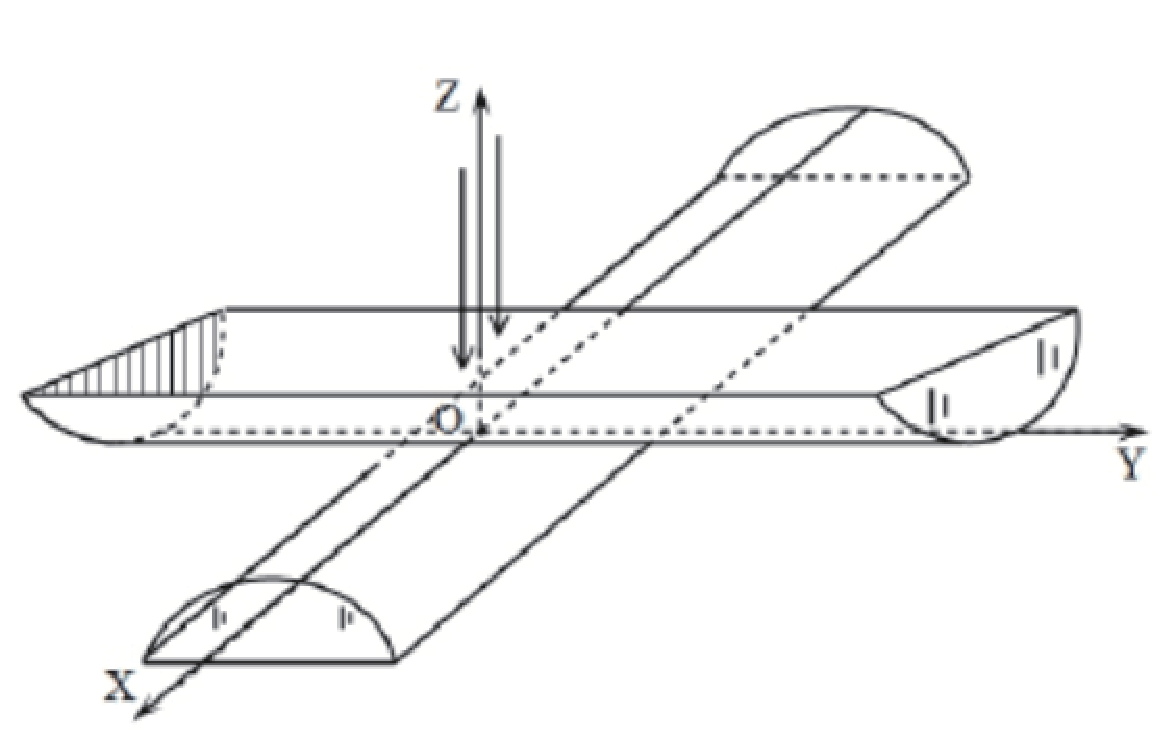
\includegraphics[width = 0.4\textwidth]{images/wave-optics-11.pdf} 
			\end{flushright}
	\tagged{student}{\vspace*{4cm}}
	\begin{taggedblock}{teacher}
		
		解析:2016复赛第一题
	\end{taggedblock}
\end{example}%%%
%%%%%%%%%%%%%%$$



\section{衍射}
 \begin{wrapfigure}{o}{4cm}
 \includegraphics[width=4cm]{images/wave-optics-6.pdf} 
 \caption{激光的衍射}
 \end{wrapfigure}
根据波动光学的惠更斯原理就可以解释,由于其波动性有机会绕过光在传播过程方向上遇到障碍物的{\heiti 衍射}(diffraction)现象,而光的电磁学说又为衍射提供了定量计算的理论基础。
由于可见光的波长非常短,只有几百纳米,所以对于通常尺度的光学现象来说,衍射效应非常之小,但当试图研究小尺度范围内的光学问题时就不得不考虑光的衍射。
完整地分析光的衍射、或一般的传播现象需要借助大量的数学计算,这里我们仅定性地分析其中的一些经典现象和简单的问题。

%%%%%%%%%%%%%%%%%
\begin{example}
试定性说明,一个透镜的最小角分辨率
\[\theta\simeq \frac{\lambda}{D},\]
其中$\lambda$是典型可见光的波长,$D$是透镜的口径。

\tagged{student}{\vspace*{4cm}}
\begin{taggedblock}{teacher}

解析:平行光通过尺度约为D的孔,可以考虑证明在偏离平行光传播方向角度$\theta \sim \frac{\lambda}{D}$处观察孔的不同部分传播到此处的相位差接近$\pi$,所以这决定了什么位置光会干涉相消,也就是小孔衍射的发散角度。透镜观察一个点,得到的像却是对透镜中心夹角接近$\theta$的光斑,所以透镜若是观察角间距小于$\theta$的两个点物将导致衍射光斑重合而无法分辨。这就是透镜的最小分辨角。
\end{taggedblock}
\end{example}
%%%%%%%%%%%%%%%%%%%%%%




%%%%%%%%%%%%%%%%%
\begin{example}

有一个口径为$100\unit{\mu m}$的He-Ne激光器,能够发射波长为$6328\pow{-10}\unit{m}$的单色光。
现将该激光器对准月球发射,试估算当激光到达月球时所覆盖的面积。
\tagged{student}{\vspace*{4cm}}
\begin{taggedblock}{teacher}

解析:\[R=\frac{\lambda L}{D}=\num{2.4e6}\si{m}\]
注意到这个衍射角度比月亮对我们的夹角还大!因为月亮半径只有$\num{1.7e6}\si{m}$。\\
面积:
\[S=\pi R^2=\num{1.8e13}\si{m}\]
\end{taggedblock}
\end{example}
%%%%%%%%%%%%%%%%%%%%%%




%%%%%%%%%%%%%%%%%
\begin{example}
某种蜜蜂的眼睛能够看到平均波长为$500\unit{nm}$的光,它是由5000个小眼构成的复眼,小眼一个个密集排放在眼睛的整个表面上,小眼构造很精巧,顶部有一个透光的圆形集光装置,叫角膜镜;下面连着圆锥形的透明晶体,使得外部入射的光线汇聚到圆锥顶点连接的感光细胞上(入射进入一个小眼的光线不会透过锥壁进入其他小眼),从而造成一个“影像点”(像素);所有小眼的影像点就拼成了一个完整的像。
若将复眼看作球面圆锥,球面半径$r=1.5\unit{mm}$,则蜜蜂小眼角膜镜的最佳直径$d$约为\kong\kong(请给出两位有效数字)。

\tagged{student}{\vspace*{2cm}}
\begin{taggedblock}{teacher}

解析:$30\unit{\mu m}$。
\end{taggedblock}
\end{example}
%%%%%%%%%%%%%%%%%%%%%%


%%%%%%%%%%%%%%%
\begin{example}
	有一个具有边长$L = 35\si{mm}$,$N_p = 5 \text{Mpix}$像素CCD感光片的数码相机,使用焦距$f = 38\si{mm}$的镜头。
	光圈的大小用一系列整数(2,2.8,4,5.6,8,11,16,22)表示,称为$F\#$,它被定义为镜头的焦距$f$与光圈口径$D$的比值$F\# = f/D$。
	
	1. 求在使用该镜头时底片上最好的空间分辨率$\Delta x_{min}$。
	
	2. 求最大的像素值,若像素超过该值将造成浪费。
	\tagged{student}{\vspace*{4cm}}
	\begin{taggedblock}{teacher}
		
		解析:1. 最大口径时衍射角最小:
		\[D_{max}=\frac{f}{2}=19\si{mm}\quad,\quad \Delta x_{min}=\frac{\lambda(\sim 500\si{nm})}{D_{max}}\cdot f=1\unit{\mu m}\]
		2. \[N_{max}=\frac{L^2}{x_{min}^2}=\num{1.2e9}\]
	\end{taggedblock}
\end{example}%%%
%%%%%%%%%%%%%%$$

%%%%%%%%%%%%%%%%%
\begin{example}

【泊松亮斑】如果让平行光垂直照射不透光的圆盘,那么在圆盘后面的光屏上留下黑影的中央将会出现一个亮斑。
试用光的波动理论解释这一现象可能的原因。
\tagged{student}{\vspace*{4cm}}
\begin{taggedblock}{teacher}

解析:略
\end{taggedblock}
\end{example}
%%%%%%%%%%%%%%%%%%%%%%

\section{偏振}
\begin{figure}
\centering
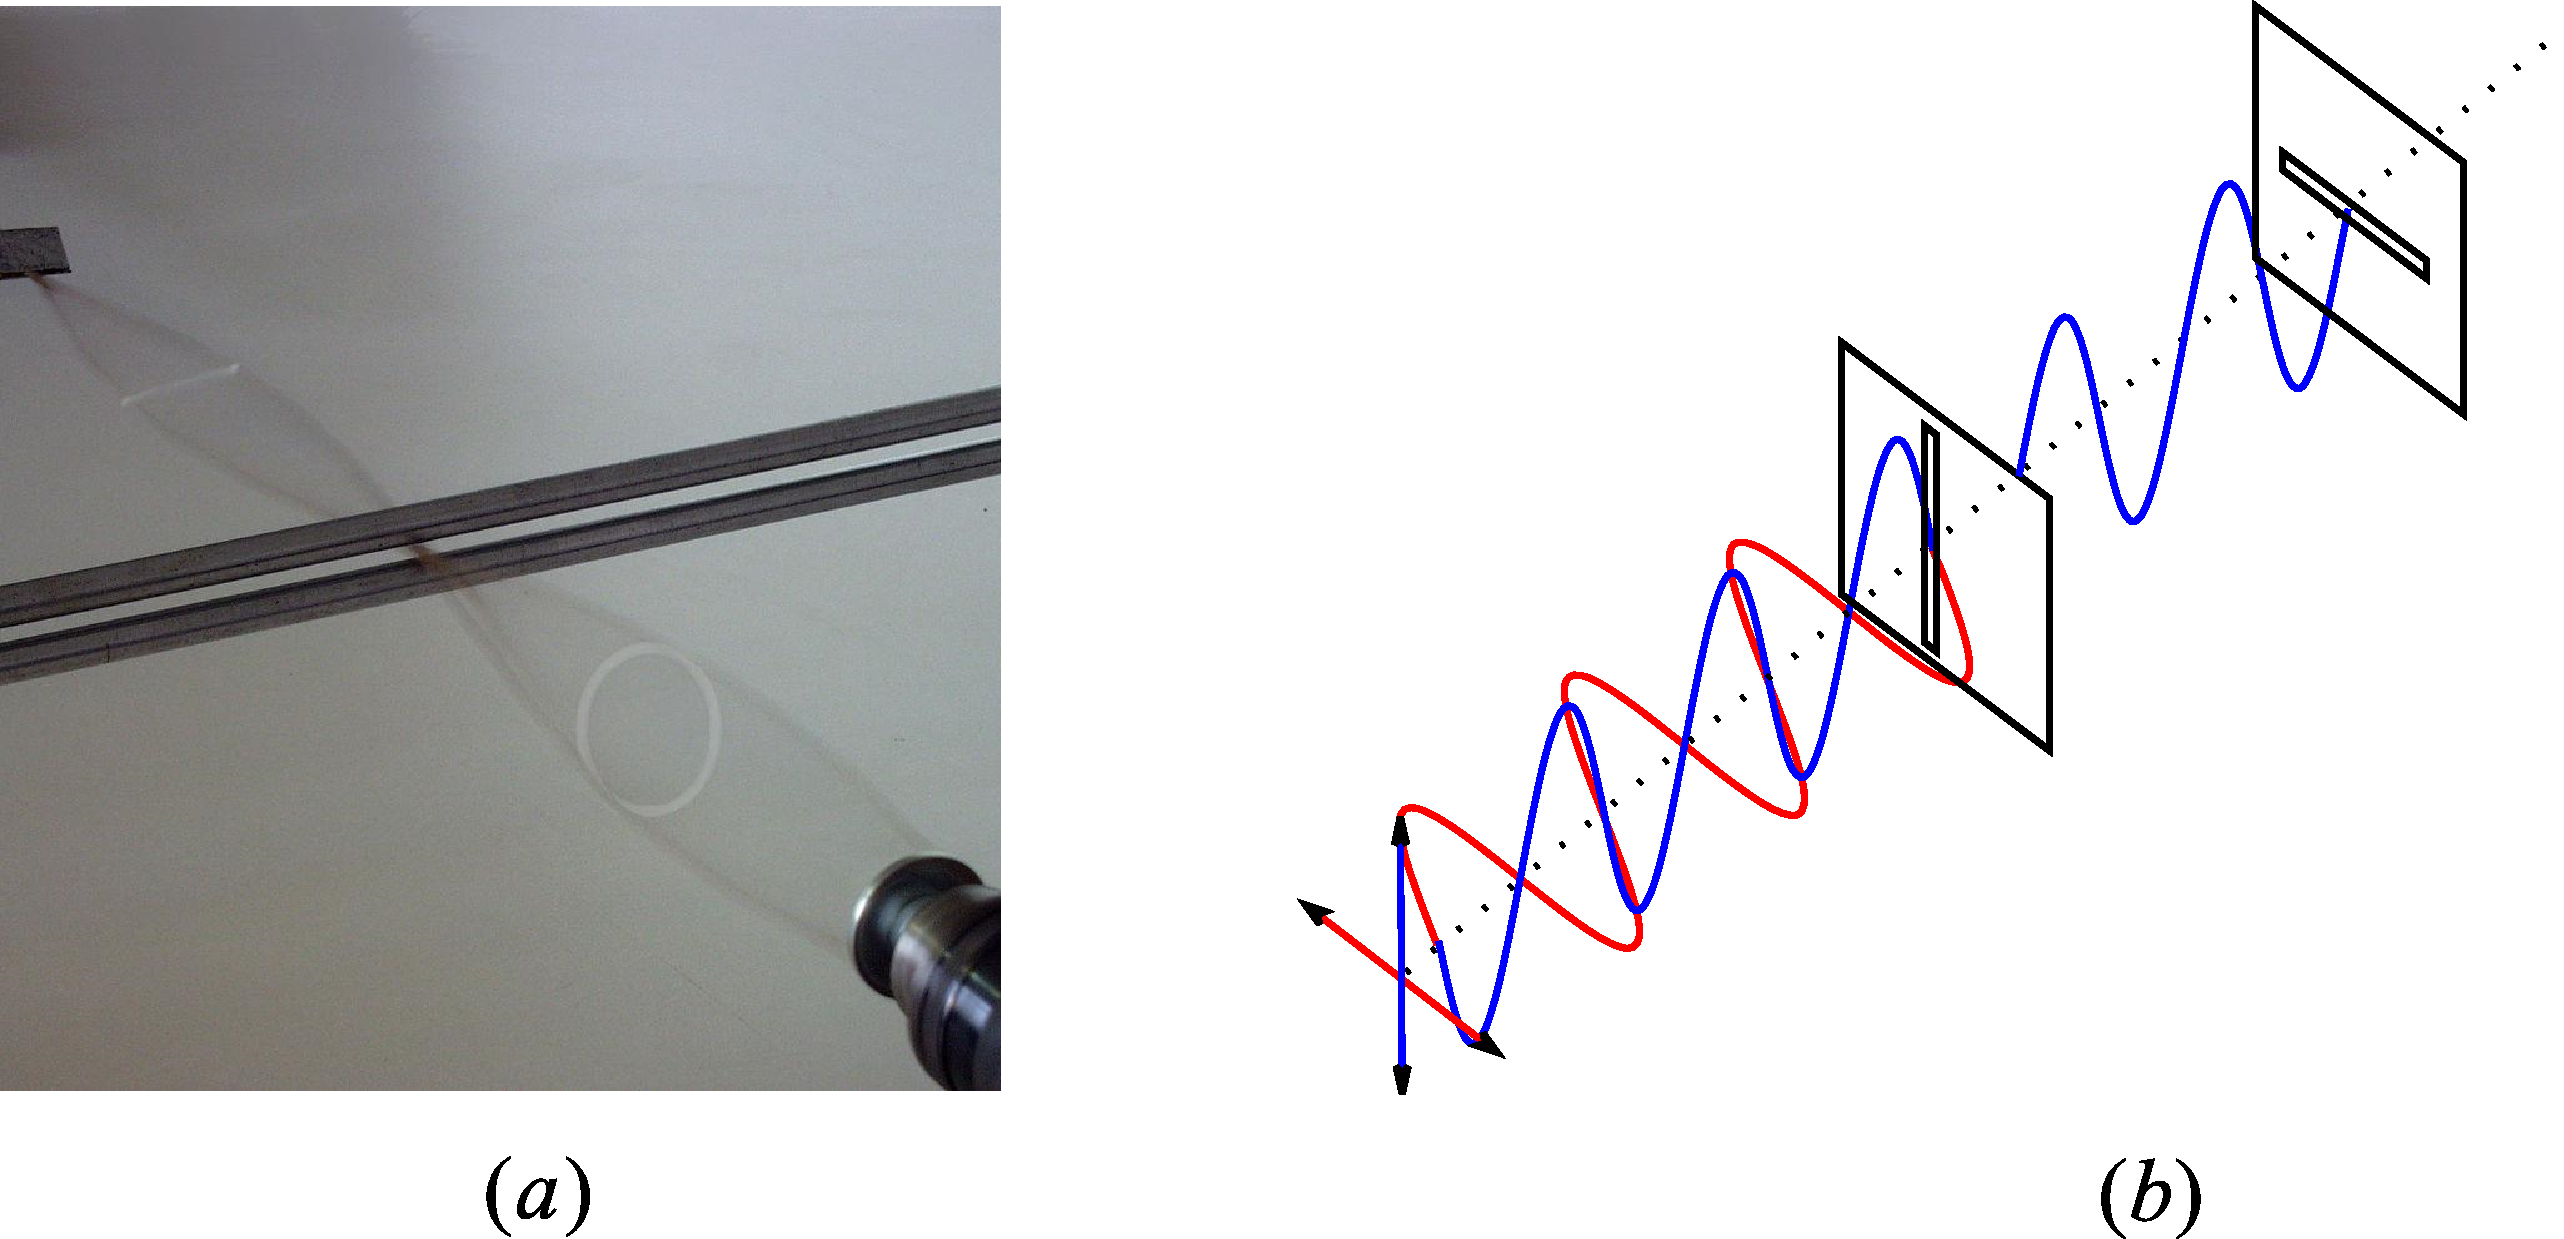
\includegraphics[width=0.8\linewidth]{images/em-theory-4}
\caption{偏振现象:(a)机械波(b)电磁波}
\label{fig:em-theory-4}
\end{figure}
前面曾经提到过,光是一种横波,也就是说它的振动方向与传播方向垂直
对于给定运动方向的平面波,垂直于传播方向是一个平面,我们知道在一个平面上有两个独立的方向,所以平面横波也存在两个独立的模式。
当平面横波的振动在空间中取特定的方向时,就称该平面波为{\heiti 线偏振波}(linear polarized wave)。
如图\ref{fig:em-theory-4}(a)所示的是机械波偏振的一个例子,振动的弦通过狭缝以后垂直于狭缝方向的振动被缝完全限制,所以在通过狭缝以后的波只剩下与缝方向一致的振动,这时就称通过缝以后得到了一个线偏振波,而图中的狭缝则被称为{\heiti 起偏器}(polarizer)。


类似的对于电磁波来说也有类似的偏振现象,如图\ref{fig:em-theory-4}(b)所示的就是光的偏振和起偏器的示意图,开始时刻的光波包含两个方向的偏振,而通过起偏器$A$之后,只有与
起偏器方向一致方向振动的电磁波才能够通过,与其垂直的方向则被阻止。
如果再放置另一个与$A$方向垂直的起偏器,简单的分析可知没有光通过再通过它,所有的光均被阻挡。
对于光来说沿着给定方向振动的偏振光还有一个专门的名称:{\heiti 线偏振光}(linear polarized light),除了线偏振以外还有另一类重要的偏振模式:{\heiti 圆偏振}(circular polarized light),现在的3D电影就是利用圆偏振光使我们看到立体影像的。
和线偏振一样,平面电磁波也可分解为两个独立的圆偏振模式,圆偏振光有左旋和右旋之分,如图\ref{fig: wave-optics-7}所示。


\begin{figure}
\centering
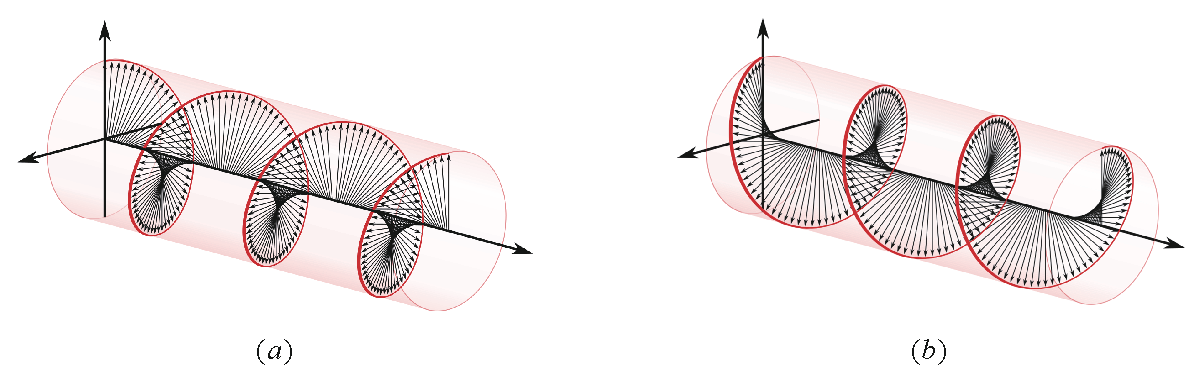
\includegraphics[width=0.8\linewidth]{images/wave-optics-7}
\caption{圆偏振:(a)左旋(b)右旋}
\label{fig: wave-optics-7}
\end{figure}



%%%%%%%%%%%%%%%%%
\begin{example}

请说明:两束偏振方向互相垂直,振幅相当,传播方向相同、相位差始终保持固定的光相遇时不会出现干涉现象。
\tagged{student}{\vspace*{4cm}}
\begin{taggedblock}{teacher}

解析:根据电磁波的叠加原理和能量正比于场强平方的事实可以得到以上结论。
\end{taggedblock}
\end{example}
%%%%%%%%%%%%%%%%%%%%%%



%%%%%%%%%%%%%%%%%
\begin{example}

试说明自然光通过偏振片后强度为入射光强的一半,忽略由于吸收、反射和散射等原因引起的光能损失。
\tagged{student}{\vspace*{4cm}}
\begin{taggedblock}{teacher}

解析:不是一半还能是什么呢?
光的能量正比于振幅,偏振方向与偏振片方向夹角为$\theta$的光通过偏振片后振幅变成了原先的$\cos\theta$,这样能量就变成了原来的$\cos^2\theta$,自然光包含了所有方向,且振幅均相同,这样通过偏振片后的能量变成原来的
\[
\frac{1}{2\pi}\int_0^{2\pi}\cos^2\theta d\theta = \frac{1}{2}.
\]
\end{taggedblock}
\end{example}
%%%%%%%%%%%%%%%%%%%%%%